\documentclass[]{article}
\usepackage{lmodern}
\usepackage{amssymb,amsmath}
\usepackage{ifxetex,ifluatex}
\usepackage{fixltx2e} % provides \textsubscript
\ifnum 0\ifxetex 1\fi\ifluatex 1\fi=0 % if pdftex
  \usepackage[T1]{fontenc}
  \usepackage[utf8]{inputenc}
\else % if luatex or xelatex
  \ifxetex
    \usepackage{mathspec}
  \else
    \usepackage{fontspec}
  \fi
  \defaultfontfeatures{Ligatures=TeX,Scale=MatchLowercase}
\fi
% use upquote if available, for straight quotes in verbatim environments
\IfFileExists{upquote.sty}{\usepackage{upquote}}{}
% use microtype if available
\IfFileExists{microtype.sty}{%
\usepackage{microtype}
\UseMicrotypeSet[protrusion]{basicmath} % disable protrusion for tt fonts
}{}
\usepackage[margin=1in]{geometry}
\usepackage{hyperref}
\hypersetup{unicode=true,
            pdftitle={Homework 5},
            pdfauthor={Noah Kawasaki},
            pdfborder={0 0 0},
            breaklinks=true}
\urlstyle{same}  % don't use monospace font for urls
\usepackage{graphicx,grffile}
\makeatletter
\def\maxwidth{\ifdim\Gin@nat@width>\linewidth\linewidth\else\Gin@nat@width\fi}
\def\maxheight{\ifdim\Gin@nat@height>\textheight\textheight\else\Gin@nat@height\fi}
\makeatother
% Scale images if necessary, so that they will not overflow the page
% margins by default, and it is still possible to overwrite the defaults
% using explicit options in \includegraphics[width, height, ...]{}
\setkeys{Gin}{width=\maxwidth,height=\maxheight,keepaspectratio}
\IfFileExists{parskip.sty}{%
\usepackage{parskip}
}{% else
\setlength{\parindent}{0pt}
\setlength{\parskip}{6pt plus 2pt minus 1pt}
}
\setlength{\emergencystretch}{3em}  % prevent overfull lines
\providecommand{\tightlist}{%
  \setlength{\itemsep}{0pt}\setlength{\parskip}{0pt}}
\setcounter{secnumdepth}{0}
% Redefines (sub)paragraphs to behave more like sections
\ifx\paragraph\undefined\else
\let\oldparagraph\paragraph
\renewcommand{\paragraph}[1]{\oldparagraph{#1}\mbox{}}
\fi
\ifx\subparagraph\undefined\else
\let\oldsubparagraph\subparagraph
\renewcommand{\subparagraph}[1]{\oldsubparagraph{#1}\mbox{}}
\fi

%%% Use protect on footnotes to avoid problems with footnotes in titles
\let\rmarkdownfootnote\footnote%
\def\footnote{\protect\rmarkdownfootnote}

%%% Change title format to be more compact
\usepackage{titling}

% Create subtitle command for use in maketitle
\newcommand{\subtitle}[1]{
  \posttitle{
    \begin{center}\large#1\end{center}
    }
}

\setlength{\droptitle}{-2em}
  \title{Homework 5}
  \pretitle{\vspace{\droptitle}\centering\huge}
  \posttitle{\par}
  \author{Noah Kawasaki}
  \preauthor{\centering\large\emph}
  \postauthor{\par}
  \predate{\centering\large\emph}
  \postdate{\par}
  \date{5/26/2018}


\begin{document}
\maketitle

\subparagraph{(a) Make time plots of the return data from 2000-01-03 to
2014-02-21. Comment on any stylized fact on returns suggested by the
plots.}\label{a-make-time-plots-of-the-return-data-from-2000-01-03-to-2014-02-21.-comment-on-any-stylized-fact-on-returns-suggested-by-the-plots.}

\includegraphics{homework_5_markdown_files/figure-latex/unnamed-chunk-1-1.pdf}
\includegraphics{homework_5_markdown_files/figure-latex/unnamed-chunk-1-2.pdf}

The stylized facts we can notice are:\\
- Mean reversion near zero\\
- Volatiltiy clustering

\subparagraph{(b) For each return series, make a four panel plot
containing a return plot, acf, density plot and normal QQ-plot. Do the
return series look normally
distributed?}\label{b-for-each-return-series-make-a-four-panel-plot-containing-a-return-plot-acf-density-plot-and-normal-qq-plot.-do-the-return-series-look-normally-distributed}

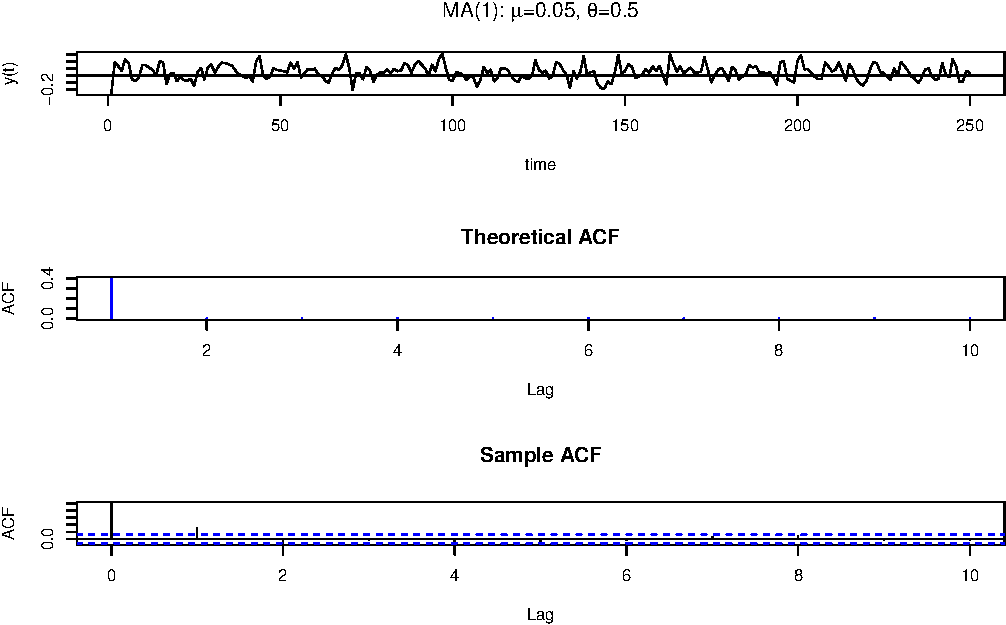
\includegraphics{homework_5_markdown_files/figure-latex/unnamed-chunk-2-1.pdf}

The ACF of the series indicates no or weak correlation across time. The
Density plot shows that it is a bell-shaped curve. However, the QQ-Plot
indicates heavier tails than a normal distribution.

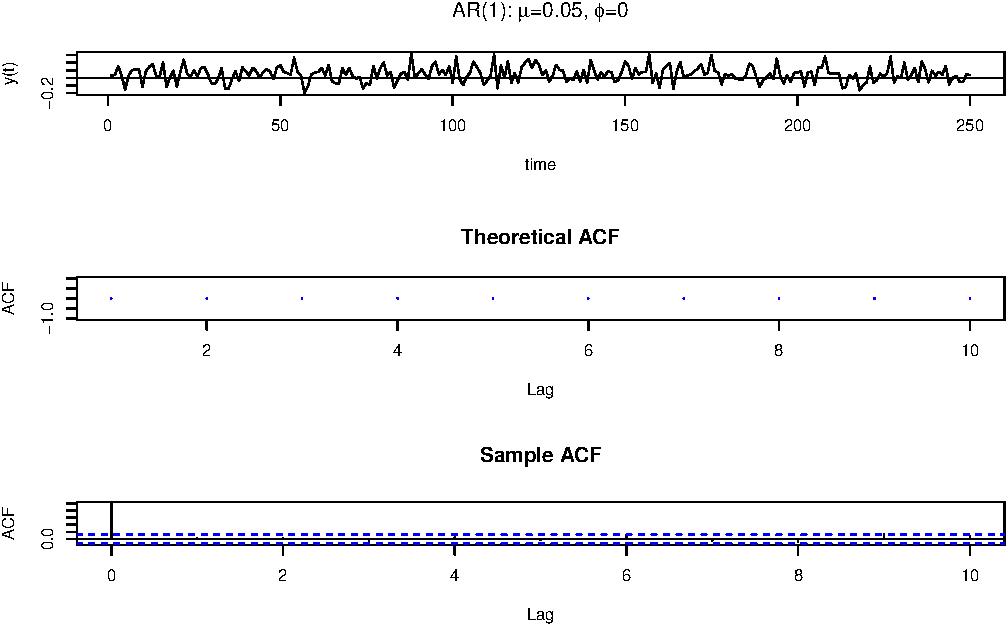
\includegraphics{homework_5_markdown_files/figure-latex/unnamed-chunk-3-1.pdf}

The ACF indicates time dependence up to order 2 lages and then some
other spikes past that the most likely do not carry economic meaning.
The density plot and QQ-Plot also indicate a bell-shaped curve with
heavier tails than a normal distribution.

\subparagraph{(c) Testing normality of each return distribution using
Jarque-Bera test
statistics.}\label{c-testing-normality-of-each-return-distribution-using-jarque-bera-test-statistics.}

\begin{verbatim}
## 
##  Jarque Bera Test
## 
## data:  MSFT.ret
## X-squared = 12100, df = 2, p-value < 2.2e-16
\end{verbatim}

\begin{verbatim}
## 
##  Jarque Bera Test
## 
## data:  GSPC.ret
## X-squared = 8847.9, df = 2, p-value < 2.2e-16
\end{verbatim}

For both series, we reject the null hypothesis that r\textsubscript{t}
is normally distributed.

\subparagraph{\texorpdfstring{(d) Now estimate GARCH(1,1) model
parameters (as in Review Questions) and report the estimated values of
\(\alpha_1\) + \(\beta_1\). How do you interpret these
results?}{(d) Now estimate GARCH(1,1) model parameters (as in Review Questions) and report the estimated values of \textbackslash{}alpha\_1 + \textbackslash{}beta\_1. How do you interpret these results?}}\label{d-now-estimate-garch11-model-parameters-as-in-review-questions-and-report-the-estimated-values-of-alpha_1-beta_1.-how-do-you-interpret-these-results}

\paragraph{(e) Plot the fitted values and the observed values. Comment
on
plots}\label{e-plot-the-fitted-values-and-the-observed-values.-comment-on-plots}

\subparagraph{\texorpdfstring{(f) For parameters \(\alpha_1\) and
\(\beta_1\) compute 95\% and (asymptotic) confidence
intervals.}{(f) For parameters \textbackslash{}alpha\_1 and \textbackslash{}beta\_1 compute 95\% and (asymptotic) confidence intervals.}}\label{f-for-parameters-alpha_1-and-beta_1-compute-95-and-asymptotic-confidence-intervals.}

\subparagraph{\texorpdfstring{(g) Test H\textsubscript{0}:
\(\alpha_1\)=0 with 95\% confidence level for each returns. Do the test
H\textsubscript{0}: \(\beta_1\)=0.9 as
well.}{(g) Test H0: \textbackslash{}alpha\_1=0 with 95\% confidence level for each returns. Do the test H0: \textbackslash{}beta\_1=0.9 as well.}}\label{g-test-h0-alpha_10-with-95-confidence-level-for-each-returns.-do-the-test-h0-beta_10.9-as-well.}

\subsubsection{MSFT}\label{msft}

\begin{verbatim}
## 
##  ***** ESTIMATION WITH ANALYTICAL GRADIENT ***** 
## 
## 
##      I     INITIAL X(I)        D(I)
## 
##      1     3.849315e-04     1.000e+00
##      2     5.000000e-02     1.000e+00
##      3     5.000000e-02     1.000e+00
## 
##     IT   NF      F         RELDF    PRELDF    RELDX   STPPAR   D*STEP   NPRELDF
##      0    1 -1.208e+04
##      1    7 -1.208e+04  2.94e-04  4.63e-04  2.0e-04  1.4e+10  2.0e-05  3.13e+06
##      2    8 -1.208e+04  1.75e-05  2.00e-05  1.9e-04  2.0e+00  2.0e-05  5.11e+01
##      3   16 -1.217e+04  7.42e-03  1.38e-02  6.0e-01  2.0e+00  1.5e-01  5.05e+01
##      4   19 -1.235e+04  1.46e-02  9.50e-03  7.3e-01  2.0e+00  3.5e-01  3.11e+00
##      5   21 -1.240e+04  3.64e-03  3.57e-03  7.8e-02  2.0e+00  7.0e-02  1.65e+03
##      6   23 -1.248e+04  6.55e-03  7.34e-03  1.3e-01  2.0e+00  1.4e-01  1.77e+05
##      7   32 -1.248e+04  1.69e-04  9.71e-04  8.5e-06  3.5e+00  1.0e-05  6.75e-02
##      8   33 -1.248e+04  1.51e-04  1.25e-04  7.9e-06  2.0e+00  1.0e-05  4.16e-02
##      9   34 -1.248e+04  4.62e-06  5.19e-06  8.5e-06  2.0e+00  1.0e-05  4.57e-02
##     10   42 -1.250e+04  1.40e-03  1.61e-03  3.2e-02  1.7e+00  4.1e-02  4.51e-02
##     11   44 -1.251e+04  9.95e-04  1.00e-03  2.9e-02  1.7e-01  4.1e-02  2.61e-03
##     12   46 -1.253e+04  9.90e-04  2.32e-03  9.1e-02  3.7e-01  1.6e-01  2.54e-03
##     13   47 -1.253e+04  1.12e-04  3.33e-03  2.0e-02  0.0e+00  3.4e-02  3.33e-03
##     14   48 -1.255e+04  2.17e-03  2.53e-03  1.0e-02  1.6e+00  1.7e-02  4.97e-03
##     15   49 -1.256e+04  7.45e-04  8.88e-04  1.5e-02  1.3e+00  3.4e-02  1.86e-03
##     16   50 -1.257e+04  3.38e-04  3.58e-04  1.4e-02  7.1e-01  3.4e-02  4.97e-04
##     17   52 -1.257e+04  5.24e-04  5.43e-04  3.1e-02  0.0e+00  6.8e-02  5.43e-04
##     18   61 -1.257e+04  2.10e-05  4.22e-04  7.9e-07  2.9e+00  1.5e-06  6.36e-04
##     19   62 -1.258e+04  1.15e-04  9.94e-05  3.5e-07  2.0e+00  7.3e-07  1.44e-04
##     20   63 -1.258e+04  1.74e-06  1.92e-06  3.3e-07  2.0e+00  7.3e-07  9.19e-06
##     21   64 -1.258e+04  2.22e-08  2.68e-08  3.2e-07  2.0e+00  7.3e-07  9.65e-06
##     22   71 -1.258e+04  4.84e-06  5.81e-06  1.3e-03  7.8e-01  3.0e-03  9.59e-06
##     23   72 -1.258e+04  1.71e-07  1.52e-06  1.2e-03  4.9e-01  3.0e-03  1.79e-06
##     24   73 -1.258e+04  6.86e-07  1.16e-06  2.4e-04  0.0e+00  5.1e-04  1.16e-06
##     25   74 -1.258e+04  1.72e-07  1.51e-07  2.4e-04  1.8e-01  5.1e-04  1.55e-07
##     26   75 -1.258e+04  6.00e-09  3.16e-09  2.5e-05  0.0e+00  4.8e-05  3.16e-09
##     27   76 -1.258e+04  2.74e-11  3.27e-12  1.3e-06  0.0e+00  3.0e-06  3.27e-12
##     28   77 -1.258e+04 -6.14e-12  1.77e-14  1.3e-07  0.0e+00  3.2e-07  1.77e-14
## 
##  ***** RELATIVE FUNCTION CONVERGENCE *****
## 
##  FUNCTION    -1.257629e+04   RELDX        1.268e-07
##  FUNC. EVALS      77         GRAD. EVALS      28
##  PRELDF       1.773e-14      NPRELDF      1.773e-14
## 
##      I      FINAL X(I)        D(I)          G(I)
## 
##      1    6.339985e-06     1.000e+00     8.826e+00
##      2    7.106840e-02     1.000e+00    -1.542e-03
##      3    9.139377e-01     1.000e+00     1.078e-03
\end{verbatim}

\begin{verbatim}
## 
## Call:
## garch(x = MSFT.ret, order = c(1, 1))
## 
## Model:
## GARCH(1,1)
## 
## Residuals:
##      Min       1Q   Median       3Q      Max 
## -11.5971  -0.5372   0.0000   0.5542   7.1233 
## 
## Coefficient(s):
##     Estimate  Std. Error  t value Pr(>|t|)    
## a0 6.340e-06   5.540e-07    11.44   <2e-16 ***
## a1 7.107e-02   4.425e-03    16.06   <2e-16 ***
## b1 9.139e-01   5.581e-03   163.75   <2e-16 ***
## ---
## Signif. codes:  0 '***' 0.001 '**' 0.01 '*' 0.05 '.' 0.1 ' ' 1
## 
## Diagnostic Tests:
##  Jarque Bera Test
## 
## data:  Residuals
## X-squared = 14357, df = 2, p-value < 2.2e-16
## 
## 
##  Box-Ljung test
## 
## data:  Squared.Residuals
## X-squared = 0.19145, df = 1, p-value = 0.6617
\end{verbatim}

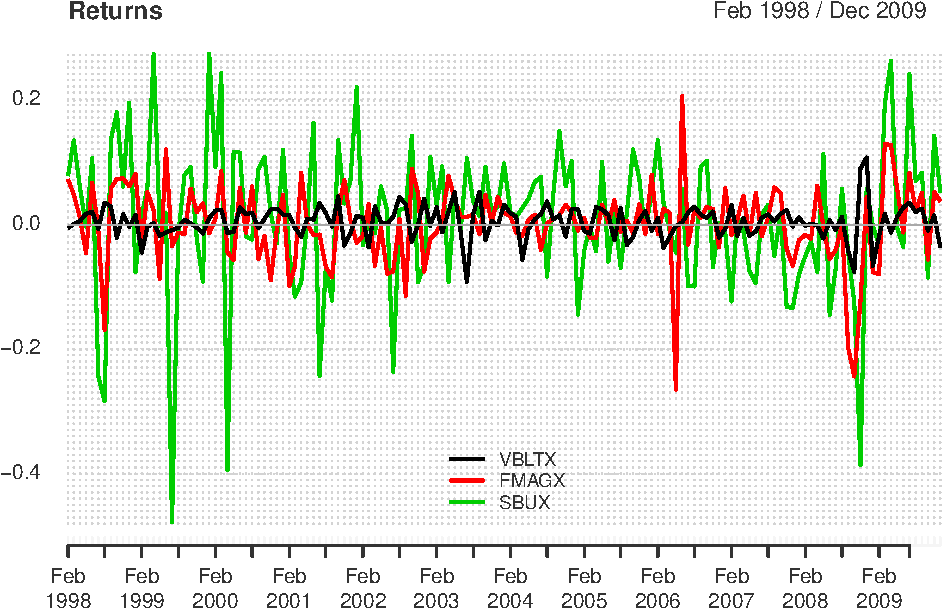
\includegraphics{homework_5_markdown_files/figure-latex/unnamed-chunk-5-1.pdf}

For MSFT, \(\omega\) = 0.000006, \(\alpha_1\) = 0.07, and \(\beta_1\) =
0.9. So \(\alpha_1\) + \(\beta_1\) = 0.97 which is very close to 1 or a
random walk process.

The fitted values and the observed values for both series look very
similar, which means the GARCH(1,1) model did a good job at explaining
our data.

\subparagraph{Confidence Intervals}\label{confidence-intervals}

\begin{verbatim}
##         a1         a1 
## 0.06239507 0.07974173
\end{verbatim}

\begin{verbatim}
##        b1        b1 
## 0.9029983 0.9248772
\end{verbatim}

\subparagraph{Hypothesis Tests}\label{hypothesis-tests}

\begin{verbatim}
##       a1 
## 16.06004
\end{verbatim}

\begin{verbatim}
##       b1 
## 2.497201
\end{verbatim}

Since both t statistics are greater than the z scores, we reject the
null hypotheses and conclude that \(\alpha_1\) \textgreater{} 0 and
\(\beta_1\) \(\neq\) 0.9.

\subsubsection{S\&P500}\label{sp500}

\begin{verbatim}
## 
##  ***** ESTIMATION WITH ANALYTICAL GRADIENT ***** 
## 
## 
##      I     INITIAL X(I)        D(I)
## 
##      1     1.547912e-04     1.000e+00
##      2     5.000000e-02     1.000e+00
##      3     5.000000e-02     1.000e+00
## 
##     IT   NF      F         RELDF    PRELDF    RELDX   STPPAR   D*STEP   NPRELDF
##      0    1 -1.373e+04
##      1    7 -1.374e+04  4.83e-04  6.95e-04  1.0e-04  9.5e+10  1.0e-05  3.32e+07
##      2    8 -1.374e+04  5.84e-05  7.26e-05  8.0e-05  2.0e+00  1.0e-05  7.23e+01
##      3    9 -1.374e+04  3.88e-06  4.08e-06  9.7e-05  2.0e+00  1.0e-05  7.15e+01
##      4   17 -1.384e+04  7.55e-03  1.24e-02  5.4e-01  2.0e+00  1.2e-01  7.10e+01
##      5   19 -1.394e+04  7.25e-03  7.32e-03  3.1e-01  2.0e+00  1.2e-01  2.75e+01
##      6   21 -1.399e+04  3.19e-03  3.09e-03  1.3e-01  2.0e+00  5.8e-02  1.30e+01
##      7   23 -1.408e+04  6.61e-03  6.31e-03  1.8e-01  2.0e+00  1.2e-01  1.38e+02
##      8   25 -1.414e+04  4.47e-03  4.50e-03  9.2e-02  2.0e+00  7.7e-02  1.62e+04
##      9   26 -1.423e+04  6.26e-03  8.99e-03  1.4e-01  2.0e+00  1.5e-01  1.36e+00
##     10   28 -1.424e+04  8.74e-04  1.13e-02  5.5e-02  1.8e+00  7.2e-02  4.73e-02
##     11   30 -1.431e+04  4.32e-03  2.97e-03  2.7e-02  1.2e+00  3.6e-02  3.77e-03
##     12   31 -1.431e+04  3.99e-04  1.32e-03  1.9e-02  8.1e-01  3.6e-02  1.70e-03
##     13   32 -1.433e+04  1.23e-03  1.81e-03  2.2e-02  1.6e+00  3.6e-02  4.68e-03
##     14   33 -1.434e+04  7.80e-04  1.79e-03  4.6e-02  2.7e-01  7.2e-02  1.87e-03
##     15   35 -1.438e+04  2.62e-03  2.24e-03  4.3e-02  0.0e+00  7.2e-02  4.56e-03
##     16   37 -1.440e+04  1.38e-03  2.25e-03  2.4e-02  2.0e+00  4.2e-02  1.02e-01
##     17   38 -1.441e+04  9.68e-04  1.62e-03  2.3e-02  1.9e+00  4.2e-02  3.05e-02
##     18   40 -1.441e+04  8.77e-05  2.01e-04  5.7e-03  1.9e+00  1.1e-02  3.68e-03
##     19   42 -1.442e+04  6.10e-04  3.86e-04  1.6e-02  0.0e+00  3.5e-02  3.86e-04
##     20   44 -1.443e+04  3.53e-04  3.67e-04  4.8e-03  1.9e+00  8.4e-03  1.38e-02
##     21   46 -1.443e+04  4.34e-04  4.64e-04  8.8e-03  6.8e-01  1.7e-02  2.15e-03
##     22   47 -1.444e+04  1.96e-04  3.22e-04  8.0e-03  1.4e+00  1.7e-02  1.26e-03
##     23   48 -1.444e+04  1.99e-04  2.60e-04  8.4e-03  8.2e-01  1.7e-02  3.49e-04
##     24   49 -1.444e+04  3.87e-06  1.21e-05  1.5e-03  0.0e+00  3.3e-03  1.21e-05
##     25   50 -1.444e+04  3.39e-06  3.38e-06  3.5e-04  0.0e+00  6.6e-04  3.38e-06
##     26   51 -1.444e+04  2.84e-09  5.28e-09  7.6e-05  0.0e+00  1.9e-04  5.28e-09
##     27   52 -1.444e+04  8.43e-10  9.82e-10  2.6e-05  0.0e+00  6.5e-05  9.82e-10
##     28   53 -1.444e+04 -1.28e-13  2.12e-15  3.8e-08  0.0e+00  9.6e-08  2.12e-15
## 
##  ***** RELATIVE FUNCTION CONVERGENCE *****
## 
##  FUNCTION    -1.443902e+04   RELDX        3.798e-08
##  FUNC. EVALS      53         GRAD. EVALS      28
##  PRELDF       2.125e-15      NPRELDF      2.125e-15
## 
##      I      FINAL X(I)        D(I)          G(I)
## 
##      1    1.553386e-06     1.000e+00     3.607e-01
##      2    8.573349e-02     1.000e+00     8.867e-04
##      3    9.035403e-01     1.000e+00    -1.723e-06
\end{verbatim}

\begin{verbatim}
## 
## Call:
## garch(x = GSPC.ret, order = c(1, 1))
## 
## Model:
## GARCH(1,1)
## 
## Residuals:
##      Min       1Q   Median       3Q      Max 
## -6.50290 -0.55024  0.06195  0.61179  3.43070 
## 
## Coefficient(s):
##     Estimate  Std. Error  t value Pr(>|t|)    
## a0 1.553e-06   2.250e-07    6.905 5.03e-12 ***
## a1 8.573e-02   6.922e-03   12.386  < 2e-16 ***
## b1 9.035e-01   7.688e-03  117.521  < 2e-16 ***
## ---
## Signif. codes:  0 '***' 0.001 '**' 0.01 '*' 0.05 '.' 0.1 ' ' 1
## 
## Diagnostic Tests:
##  Jarque Bera Test
## 
## data:  Residuals
## X-squared = 269.44, df = 2, p-value < 2.2e-16
## 
## 
##  Box-Ljung test
## 
## data:  Squared.Residuals
## X-squared = 8.6754, df = 1, p-value = 0.003225
\end{verbatim}

\includegraphics{homework_5_markdown_files/figure-latex/unnamed-chunk-8-1.pdf}

For S\&P500, \(\omega\) = 0.0000015, \(\alpha_1\) = 0.086, and
\(\beta_1\) = 0.9. So \(\alpha_1\) + \(\beta_1\) = 0.98 which is also
very close to 1 or a random walk process.

The fitted values and the observed values for both series look very
similar, which means the GARCH(1,1) model did a good job at explaining
our data.

\subparagraph{Confidence Intervals}\label{confidence-intervals-1}

\begin{verbatim}
##         a1         a1 
## 0.07216643 0.09930056
\end{verbatim}

\begin{verbatim}
##        b1        b1 
## 0.8884712 0.9186094
\end{verbatim}

\subparagraph{Hypothesis Tests}\label{hypothesis-tests-1}

\begin{verbatim}
##       a1 
## 12.38571
\end{verbatim}

\begin{verbatim}
##       b1 
## 0.460477
\end{verbatim}

\(\alpha_1\) is greater than its z score but \(\beta_1\) is less than
its z score so we reject the null for \(\alpha_1\) and conclude that
\(\alpha_1\) \textgreater{} 0 but fail to reject for \(\beta_1\) and
conclude that \(\beta_1\) = 0.9.


\end{document}
